\documentclass{ansarticle-preprint}
\PassOptionsToPackage{loadshadow}{todonotes}
%\usepackage{ucs}
\usepackage[utf8]{inputenc}
\usepackage{amsmath}
%\usepackage{cite}
\usepackage{anslistings}
\usepackage{multicol}
\usepackage{pdfsync}
\usepackage{enumitem}

\usepackage{pgfplots}
\usepackage{pgfplotstable}

\usepackage{fontenc}
\usepackage{graphicx}
\usepackage{xspace}

\usepackage{siunitx}

\usepackage{floatflt}

\usepackage{multirow}

\usepackage{booktabs}

%\renewcommand{\baselinestretch}{2.0}
%\usepackage{lineno}
%\renewcommand\linenumberfont{\normalfont\tiny}
%\linenumbers

\graphicspath{{svg/}}

\usepackage[normalem]{ulem}

\usepackage{caption}
\usepackage{subcaption}

\setlength{\marginparwidth}{2cm}

\pgfplotsset{compat=1.9}
\definecolor{gnuplot@lightblue}{RGB}{87,181,232}
\definecolor{gnuplot@green}{RGB}{0,158,115}
\definecolor{gnuplot@purple}{RGB}{148,0,212}

\newcommand{\specialword}[1]{\texttt{#1}}
\newcommand{\dealii}{{\specialword{deal.II}}\xspace}
\newcommand{\pfrst}{{\specialword{p4est}}\xspace}
\newcommand{\trilinos}{{\specialword{Trilinos}}\xspace}
\newcommand{\aspect}{\specialword{Aspect}\xspace}
\newcommand{\petsc}{\specialword{PETSc}\xspace}
\newcommand{\snes}{{\specialword{SNES}}\xspace}
\newcommand{\ts}{{\specialword{TS}}\xspace}
\newcommand{\petscsf}{{\specialword{SF}}\xspace}
\newcommand{\cmake}{{\specialword{CMake}}\xspace}
\newcommand{\candi}{{\specialword{candi}}\xspace}
\newcommand{\MPI}{{\specialword{MPI}}\xspace}
\newcommand{\MPIx}{{\specialword{MPI+X}}\xspace}
\newcommand{\sundials}{{\specialword{SUNDIALS}}\xspace}
\newcommand{\kinsol}{{\specialword{KINSOL}}\xspace}
\newcommand{\ida}{{\specialword{IDA}}\xspace}
\newcommand{\arkode}{{\specialword{ARKODE}}\xspace}
\newcommand{\boost}{{\specialword{Boost}}\xspace}
\newcommand{\kokkos}{{\specialword{Kokkos}}\xspace}
\newcommand{\llvm}{{\specialword{LLVM}}\xspace}
\newcommand{\step}[1]{{\specialword{step-#1}}\xspace}

%Trilinos Packages
\newcommand{\epetra}{{\specialword{Epetra}}\xspace}
\newcommand{\petra}{{\specialword{Petra}}\xspace}
\newcommand{\teuchos}{{\specialword{Teuchos}}\xspace}
\newcommand{\tpetra}{{\specialword{Tpetra}}\xspace}


\usetikzlibrary{shapes.misc,shadows}
\tikzset{cross/.style={cross out, draw=black, minimum size=2*(#1-\pgflinewidth), inner sep=0pt, outer sep=0pt},
%default radius will be 1pt.
cross/.default={2pt}}

%
% Author list -- please add yourself in both places below (in
%                alphabetical order) if you think that your
%                contributions to the last release warrant this
%

\hypersetup{
  pdfauthor={
    Daniel Arndt,
    Wolfgang Bangerth,
    Bruno Blais,
    Marc Fehling,
    Rene Gassm\"{o}ller,
    Timo Heister,
    Luca Heltai,
    Vladimir Ivannikov,
    Martin Kronbichler,
    Matthias Maier,
    Peter Munch,
    Andreas Steger,
    Dominik Still,
    Bruno Turcksin,
    David Wells
  },
  pdftitle={The deal.II Library, Version 9.8},
}

\title{The \dealii Library, Version 9.8}

 \author[1*]{Daniel Arndt}
 \affil[1]{Computational Coupled Physics Group,
   Computational Sciences and Engineering Division,
   Oak Ridge National Laboratory, 1 Bethel Valley Rd.,
   TN 37831, USA.
   \texttt{arndtd/turcksinbr@ornl.gov}}

 \author[2,3]{Wolfgang~Bangerth}
 \affil[2]{Department of Mathematics, Colorado State University, Fort
   Collins, CO 80523, USA.
   \texttt{bangerth@colostate.edu}}
 \affil[3]{Department of Geosciences, Colorado State University, Fort
   Collins, CO 80523, USA.}

\author[4]{Bruno Blais}
\affil[4]{Chemical Engineering High-performance Analysis, Optimization and Simulation (CHAOS) laboratory, Department of Chemical Engineering,
             Polytechnique Montréal,
             PO Box 6079, Stn Centre-Ville, Montréal, Québec, Canada, H3C 3A7.
             {\texttt{bruno.blais@polymtl.ca}}}

\author[5]{Marc~Fehling}
\affil[5]{Department of Mathematical Analysis,
    Faculty of Mathematics and Physics, Charles University,
    Sokolovsk{\'a} 49/83, 186\,75 Prague 8, Czech Republic.
    {\texttt{marc.fehling@matfyz.cuni.cz}}}


\author[6]{Rene~Gassm\"{o}ller}
\affil[6]{GEOMAR Helmholtz Centre for Ocean Research Kiel, 24148 Kiel, Germany.
   {\texttt{rgassmoeller@geomar.de}}}

\author[7]{Timo~Heister}
\affil[7]{School of Mathematical and Statistical Sciences,
   Clemson University,
   Clemson, SC, 29634, USA.
   {\texttt{heister@clemson.edu}}}

\author[8]{Luca~Heltai}
\affil[8]{Department of Mathematics, University of Pisa,
Via Buonarroti 1/c, 56127 Pisa, Italy. {\texttt{luca.heltai@unipi.it}}}

\author[9]{Vladimir~Ivannikov}
\affil[9]{Institute of Material Systems Modeling, Helmholtz-Zentrum Hereon,
Max-Planck-Stra{\ss}e 1, 21502 Geesthacht, Germany. {\texttt{vladimir.ivannikov@hereon.de}}}

\author[10]{Martin~Kronbichler}
\affil[10]{Faculty of Mathematics, Ruhr University Bochum,
   Universit\"atsstr.~150, 44780 Bochum, Germany.
 {\texttt{martin.kronbichler@rub.de}}}

\author[11]{Matthias~Maier}
\affil[11]{Department of Mathematics,
  Texas A\&M University,
  3368 TAMU,
  College Station, TX 77845, USA.
  {\texttt{maier@math.tamu.edu}}}

\author[12]{Peter Munch}
\affil[12]{Institute of Mathematics, Technical University of Berlin, Germany.
  {\texttt{muench@math.tu-berlin.de}}}

\author[13]{Andreas Steger}
\affil[13]{TUM School of Engineering and Design, Technical University of Munich, Germany.
  {\texttt{andreas.steger@tum.de}}}

\author[14]{Dominik Still}
\affil[14]{Institute for Computational Mechanics, TUM School of Engineering and Design, Technical
University of Munich, Germany.
  {\texttt{dominik.still@tum.de}}}

\author[1*]{Bruno~Turcksin}

\author[15]{David Wells}
\affil[15]{Department of Mathematics, University of North Carolina,
  Chapel Hill, NC 27516, USA.
  {\texttt{drwells@email.unc.edu}}}

\renewcommand{\labelitemi}{--}


\begin{document}
\maketitle

\footnotetext{%
  $^\ast$ This manuscript has been authored by UT-Battelle, LLC under Contract No.
  DE-AC05-00OR22725 with the U.S. Department of Energy.
  % We need to submit the manuscript with the text below. If the editor
  % complains we can remove it.
  The United States
  Government retains and the publisher, by accepting the article for
  publication, acknowledges that the United States Government retains a
  non-exclusive, paid-up, irrevocable, worldwide license to publish or reproduce
  the published form of this manuscript, or allow others to do so, for United
  States Government purposes. The Department of Energy will provide public
  access to these results of federally sponsored research in accordance with the
  DOE Public Access Plan (http://energy.gov/downloads/doe-public-access-plan).
}


\begin{abstract}
  This paper provides an overview of the new features of the finite element
  library \dealii, version 9.8.
\end{abstract}



%%%%%%%%%%%%%%%%%%%%%%%%%%%%%%%%%%%%%%%%%%%%%%%%%%%%%%%%%%%%%%%%%%%%%%%%%%%%%%%%
%%%%%%%%%%%%%%%%%%%%%%%%%%%%%%%%%%%%%%%%%%%%%%%%%%%%%%%%%%%%%%%%%%%%%%%%%%%%%%%%
%%%%%%%%%%%%%%%%%%%%%%%%%%%%%%%%%%%%%%%%%%%%%%%%%%%%%%%%%%%%%%%%%%%%%%%%%%%%%%%%
\section{Overview}

\dealii version 9.8.0 was released XXX.
\todo{All: Fill in release date once known}
This paper provides an overview of the new features of this release and
serves as a citable reference for the \dealii software library version 9.8.
\dealii is an object-oriented finite element library used around the world
in the development of finite element solvers. It is available under the
terms of the \emph{Apache License 2.0\footnotemark[1] with LLVM
Exception\footnotemark[2]} and separately under the terms of the \emph{GNU
Lesser General Public License v2.1.\footnotemark[3]}
Downloads are available at \url{https://www.dealii.org/} and
\url{https://github.com/dealii/dealii}.
%
\footnotetext[1]{\url{https://spdx.org/licenses/Apache-2.0.html}}
\footnotetext[2]{\url{https://spdx.org/licenses/LLVM-exception.html}}
\footnotetext[3]{\url{https://spdx.org/licenses/LGPL-2.1-or-later.html}}

The major changes of this release are:
%
\begin{itemize}
\item Substantially extended support for meshes that contain
  triangles, tetrahedra, wedges, and pyramids (see
  Section~\ref{subsec:non-hypercube}).
\item Improved support for and performance on GPUs (see
  Section~\ref{subsec:gpu}).
\item Support for newer versions of Trilinos that build on its newer
  Tpetra, rather than the older Epetra, foundation (see
  Section~\ref{subsec:tpetra}).
\item Much extended interfaces to the VTK library (see
  Section~\ref{subsec:vtk}) and the SUNDIALS library (see
  Section~\ref{subsec:arkode}).
\item A lot of work on reducing memory allocations to improve
  performance (see Section~\ref{subsec:memory}).
\item Continued evolution alongside newer C++ standards (see
  Section~\ref{subsec:cxx}).
\item A substantial number of new tutorial and code gallery programs
  (see Section~\ref{subsec:steps}).
\end{itemize}
%



While all of these major changes are discussed in detail in
Section~\ref{sec:major}, there
are a number of other noteworthy changes in the current \dealii release,
which we briefly outline in the remainder of this section:
%
\begin{itemize}
\item Major parts of the \texttt{MeshWorker} framework are now
  deprecated. When originally written, more than 20 years ago,
  \texttt{MeshWorker} was an attempt at automatizing many parts of
  what a finite element code does. It succeeds at making easy things
  easier, but makes it very difficult to transition, for example, from a
  discretization of a simple PDE without coefficients to a real
  problem with nonlinearities, spatially variable coefficients, and
  similar things. It was also never well documented or tested, and
  only \step{39} heavily relied on it. \step{39} has now been rewritten,
  and all of the classes it used are now deprecated. The only piece
  within the \texttt{MeshWorker} namespace that will survive in the
  long run is the \texttt{MeshWorker::mesh\_loop()} function and its
  dependencies.
\item Our wrappers of PETSc's linear algebra classes now support multi-threaded assembly into and reading from vectors ghost.
\item We have extended the matrix-free infrastructure for the
  evaluation and integration of N{\'e}d{\'e}lec elements.
\item The internal representation of imposing Dirichlet boundary conditions in
  the matrix-free infrastructure was reworked and made more similar between
  the GPU and CPU implementations, leading to faster execution on most CPU
  systems.
\end{itemize}
%
The
\href{https://dealii.org/developer/doxygen/deal.II/changes_between_9_7_1_and_9_8_0.html}{changelog}
-- listing more than 140
new features and bugfixes --
contains a complete record of all changes; see \cite{changes98}.



%%%%%%%%%%%%%%%%%%%%%%%%%%%%%%%%%%%%%%%%%%%%%%%%%%%%%%%%%%%%%%%%%%%%%%%%%%%%%%%%
%%%%%%%%%%%%%%%%%%%%%%%%%%%%%%%%%%%%%%%%%%%%%%%%%%%%%%%%%%%%%%%%%%%%%%%%%%%%%%%%
%%%%%%%%%%%%%%%%%%%%%%%%%%%%%%%%%%%%%%%%%%%%%%%%%%%%%%%%%%%%%%%%%%%%%%%%%%%%%%%%
\section{Major changes to the library}
\label{sec:major}

This release of \dealii contains a number of large and significant changes,
which we will discuss in the following.


%%%%%%%%%%%%%%%%%%%%%%%%%%%%%%%%%%%%%%%%%%%%%%%%%%%%%%%%%%%%%%%%%%%%%%%%%%%%%%%%

\subsection{Support for meshes with non-hypercube cells}
\label{subsec:non-hypercube}

We have continued \dealii{}'s transition from a library that
historically only
supported hypercube cells to one that also supports triangular (in
2d), tetrahedral, pyramidal, and wedge-shaped cells (in 3d) meshes, as well
as mixed meshes. In particular, we have put substantial effort into
supporting more finite element types on these meshes.

The pyramid finite elements \texttt{FE\_PyramidP} and \texttt{FE\_PyramidDGP} now support quadratic and cubic shape functions, extending the mixed-mesh capabilities introduced in release 9.3~\cite{dealII93} to higher polynomial orders.
The underlying approximation space is constructed by transforming the
orthogonal basis of Bergot et al.~\cite{Bergot2010} into a nodal Lagrange basis.
Analogous constructions are implemented for simplices and wedges.
The orthogonal basis functions are expressed in terms of (homogenized) Jacobi polynomials and evaluated using recurrence relations rather than explicit polynomial expressions.
Derivatives are evaluated using the same recurrence-based approach, avoiding computations at singularities while improving numerical stability.
The pyramid basis functions form an exception, as their approximation space is spanned by rational rather than polynomial functions.

The introduction of second- and third-order nodal pyramid elements requires support for degrees of freedom located on edges and faces for mixed element types.
To ensure a consistent distribution of the DoFs across interfaces, the \textit{hp}-infrastructure has been extended to account for the different face topologies on transitional elements, thereby preserving continuity on conforming meshes.

Increasing the polynomial degree of the shape functions also requires quadrature rules of sufficiently high order to consistently evaluate weak-form integrals, particularly in the presence of non-linear terms or curvilinear mappings.
To this end, mixed-mesh computations are supported by Stroud quadrature rules.
These rules provide integration formulas of arbitrary order and serve as a fallback whenever no alternative quadrature rule of sufficient accuracy is available.

Additionally, isotropic refinement is now supported for pyramids and
wedges. The underlying algorithms employ a midpoint refinement
strategy similar to the one used for hexahedra and tetrahedra. It
recursively subdivides a cell's constituent lower-dimensional entities
-- from lines to faces, and finally to the element itself. This hierarchical approach ensures mesh conformity across neighboring elements. Under this scheme, an isotropic refinement step partitions a pyramid into ten and a wedge into eight children.

As an alternative to working directly with simplex meshes, \dealii now
provides the function
\texttt{GridGenerator::convert\_simplex\_to\_hypercube\_mesh()}, which
converts a simplex mesh into a pure hypercube mesh.
In two dimensions, each triangle is subdivided into three quadrilaterals by inserting a vertex at the barycenter and connecting it to the edge midpoints.
In three dimensions, each tetrahedron is decomposed into four hexahedra by applying the same subdivision to every face and adding a vertex at the tetrahedron's barycenter.

To enable the evaluation of finite element fields across interfaces in
mixed meshes, the class \texttt{FEInterfaceValues} now supports heterogeneous element types.
The two sides of a face or subface may use different finite elements, mappings, and quadrature rules, even allowing for adaptively refined mixed meshes in two dimensions.

\subsection{Performance Portable GPU support}
\label{subsec:gpu}

This release comes with numerous new features, fixes, and performance improvements for running on GPUs, making GPUs
usable in practice to speed up computations.

We build on Kokkos \cite{trott2022} for performance portability, meaning a
code written based on the \texttt{Portable::MatrixFree} classes can run on
current GPUs from NVIDIA, AMD, and Intel without any vendor-specific code
visible in the user code. Importantly, all functionality is also available
on the CPU if \dealii{} is configured without GPU support.

A representative use case is the new \step{104} tutorial program (see also
Section~\ref{subsec:steps}), that solves the Stokes equation using a block
preconditioner and an inner geometric multigrid V-cycle. The operator
evaluation and multigrid cycle is running without assemblying any matrices
(i.e., ``matrix-free''). Performance results for a variety of GPUs and CPUs
are presented in Table~\ref{fig:step-104b}.

\begin{table}[tbp]
 \caption{\it Stokes operator throughput and time to solve the system
   for different devices. PMF denotes the new \texttt{Portable::MatrixFree}
   implementation optimized for GPUs, and MF denotes the CPU-based
   \texttt{MatrixFree} framework leveraging SIMD. MF$_{\text{ir}}$ is a
   less optimized variant of MF that runs on distorted meshes. Results from
   step-104, on a problem with 53 million degrees of freedom, in 3D.}
 \label{fig:step-104b}

\centering
  \begin{tabular}{lllrrrrr}
    \toprule
    \bfseries Name & & & \bfseries FP64 & \bfseries VRAM & \bfseries BW & \bfseries Operator & \bfseries Solve Time \\
    & & & [TFLOPS] & [GB] & [TB/s] & [MDoFs/s] & [s]
    \\[0.5em]
    AMD W7800       & GPU & PMF              & 1.41 & 32 & 0.6 & 469 & 31     \\
    NVIDIA RTX 6000 & GPU & PMF              & 1.97 & 96 & 1.8 & 1{,}746 & 11 \\
    NVIDIA H100     & GPU & PMF              & 25.6 & 80 & 3.4 & 1{,}457 & 9
    \\[0.25em]
    % single processor setup:
    AMD 5975WX      & CPU & PMF              & 2.0 & -- & 0.2 & 113 & 135 \\
    AMD 5975WX      & CPU & MF               & 2.0 & -- & 0.2 & 1,873 & 13 \\
    AMD 5975WX      & CPU & MF$_{\text{ir}}$ & 2.0 & -- & 0.2 & 995 & 21
    \\[0.25em]
    % dual processor setup:
    % 12.7 TFLOPs is theoretical max, 11.9 TFLOPs seem to be observed in the wild
    % 0.92TB/s theoretical memory bandwidth, 0.78TB/s seems to be observed in the wild
    2x AMD EPYC 9754   & CPU & PMF              & 12.7 & -- & 0.92 &      654 & 26 \\ % 25.74s
    2x AMD EPYC 9754   & CPU & MF               & 12.7 & -- & 0.92 & 12{,}129 & 3  \\ % 2.846s
    2x AMD EPYC 9754   & CPU & MF$_{\text{ir}}$ & 12.7 & -- & 0.92 &  4{,}885 & 5  \\ % 4.933s
    \bottomrule
  \end{tabular}
  \\[0.25em]
\end{table}

Similar to the \texttt{MatrixFree} framework designed for CPUs,
throughput for operator evaluation increases with polynomial
degree. This is in contrast to matrix-vector products using assembled
matrices that get slower the higher the finite element degree, as more
entries per row are nonzero. As GPUs are highly parallel devices, a
significant number of unknowns per GPU are required to reach peak
performance, as is clear from Figure~\ref{fig:step-104}.





\begin{figure}[tbp]
 \centering
 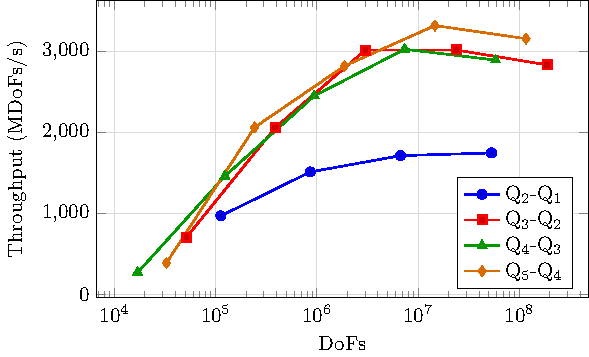
\includegraphics{step-104/plots-figure0.pdf}
 %
 \caption{\it Throughput of a Stokes operator application for
   different problem sizes and finite element degrees on an NVIDIA RTX
   6000 Blackwell Max-Q GPU. The \step{104} program provides a
   detailed description and more performance data.}
 \label{fig:step-104}
\end{figure}



The new tutorial showcases various new features of \dealii{}:
First, \texttt{Portable::MatrixFree} now supports systems of
equations by allowing for the use of more than one \texttt{Portable::FEEvaluation} object within an operator. In
\step{104}, this is used to define the Stokes operator with a
velocity and pressure evaluation object using the same quadrature
rule.
Secondly, we overhauled the interface by providing \texttt{DeviceVector} and \texttt{DeviceBlockVector} classes
within the matrix-free GPU kernels instead of exposing raw C-style
pointers.
Thirdly, the complete geometric multigrid cycle including multigrid
transfer for $h$ and $p$ coarsening runs on device without copying solution data between host and GPU, even when running with multiple GPUs. This is achieved using device-aware MPI support.
Fourth, performance has been significantly improved by code optimizations, reducing the number
of GPU fences, and by using multithreading for setup steps that run on the CPU.

Finally, usability improved with various additional error checks throughout the interface, improved API documentation, and other new features. Taken together, the work over the last twelve months makes the portable matrix-free framework a competitive solution for
performance critical \dealii{} applications.

\todo[inline]{Timo/Martin: Comparing the 4th and 5th rows of the
  table, it seems like PMF is still slower than MF by a factor of
  3-4. Do you want to write a paragraph that discusses this
  discrepancy and/or outline future plans to address it?}

\todo[inline]{Short reply by Martin: I do not think we can close the gap
  between PMF and MF in the near future, because the abstractions of PMF are
  not well-suited for CPUs (we are trying hard to make them work well for
  GPUs, and by the work of several people, we have made good progress already
  and will make more). So indeed, we should describe these differences, and
  maybe point to higher-level plans I have to encapsulate such cases more
  abstractly into global operators. Timo, if you agree I will write such a
  paragraph, and you can fill the parts I'm missing.}

\subsection{Trilinos and Tpetra interfaces}
\label{subsec:tpetra}

The \trilinos{} project is an important
dependency for \dealii{}, providing one way
to parallel linear algebra classes as well as numerous other pieces of
functionality like solvers and preconditioners. Historically, Trilinos has
provided parallel linear algebra functionality through its \epetra{}
sub-packages. However, the \trilinos{} project has long intended
to replace their \epetra{}-based solver stack in favor of
\tpetra{}-based solvers. Support for different number
types and \texttt{Kokkos} execution spaces has been the main
driver of this transition, the latter also enabling support for GPUs or other
acceleration devices. The \epetra{}-based stack was finally removed
in the recent \trilinos{} 17 release. Because \dealii{}'s
Trilinos wrappers were all based on \epetra{}, this
has required us to complete the \tpetra{} wrappers we had
started to write in recent years; for example, the
\texttt{TpetraWrappers::Vector} class has been available since \dealii{}
9.1, and a basic implementation for
\texttt{TpetraWrappers::SparsityPattern} and
\texttt{TpetraWrappers::SparseMatrix} was included in the 9.6
\dealii release. However, much functionality was still missing,
and in particular \dealii would not configure
and compile with \trilinos{} if the \epetra{} stack was not present.

With \dealii 9.8 \tpetra{} support was expanded
significantly, while simultaneously improving the compatibility between \tpetra{} and
\epetra based wrapper classes. We now support \trilinos{}
versions that include the \epetra{}-based stack, the \tpetra{}-based stack,
or both; in particular, this includes
\trilinos{}' latest release 17 that no longer has \epetra{} support.
In case \epetra{} is available, the \texttt{TrilinosWrappers} namespace
continues to use \epetra{} but will use \tpetra{}
if only \tpetra{} is available. The \texttt{TpetraWrappers}
namespace will always use \tpetra{} and is only available if
\trilinos{} was configured with \tpetra{}.

While we generally expect the \tpetra{}
stack to work, not all functionality from namespace
\texttt{TrilinosWrap\allowbreak{}pers} is available in the
\texttt{TpetraWrappers} namespace at this time. However, in practice we
built very large packages with the \tpetra{} wrappers,
indicating that all \textit{major} functionality is available. On the
other hand, a substantial number of our Trilinos wrapper tests and
several of \dealii{}'s example programs fail when
run against the \tpetra{} wrappers, suggesting that some
functionality available in our \epetra{} wrappers are not
yet implemented in the \tpetra{} wrappers.


\subsection{VTK interfaces}
\label{subsec:vtk}

The interfaces in the \texttt{VTKWrappers} namespace have been
substantially extended.  The new functionality provides a bidirectional
bridge between VTK data sets and the mesh, finite-element, and vector
abstractions used by \dealii.  In particular, VTK files can now be read in
stages: \texttt{read\_tria()} constructs a \texttt{Triangulation}, while
\texttt{read\_cell\_data()} and \texttt{read\_vertex\_data()} expose data
associated with cells and vertices, respectively.  The corresponding
\texttt{read\_all\_data()} utility collects all data arrays into a single
serial vector, and \texttt{read\_vtk()} provides a combined interface for
loading a VTK file and its associated finite-element data.

The description of the data in a VTK file can also be translated into a
compatible \dealii{} finite-element object with
\texttt{vtk\_to\_finite\_element()}.  This makes it possible to preserve
the number and location of the degrees of freedom represented in the file
without imposing an interpretation on multi-component arrays.  Once a
\texttt{DoFHandler} has been constructed, \texttt{data\_to\_dealii\_vector()}
maps the VTK data onto a \dealii{} vector, including distributed vectors on a
parallel triangulation.  The supporting
\texttt{GridTools::parallel\_to\_serial\_vertex\_indices()} utility supplies
the vertex-numbering correspondence required when data are read on a
serial mesh and then transferred to a distributed one.

Finally, the VTK interface now supports two-way conversion between a
\texttt{Triangulation} and a \texttt{vtkUnstructuredGrid}.  This allows
meshes to be exchanged with VTK-based visualization and meshing tools in
both directions, including meshes with non-hypercube reference-cell
types supported by the library.  The conversion optionally transfers
manifold, boundary, and material identifiers associated with the \dealii{}
mesh.  Together, these additions make it possible to use VTK files as input for restarting or
preprocessing computations while retaining the topology and metadata
needed by a finite-element program.


\subsection{Interfaces to the SUNDIALS ARKODE package}
\label{subsec:arkode}

The interfaces to the \texttt{SUNDIALS} \texttt{ARKODE} package have
been substantially reorganized, now matching the internal organization
of \texttt{ARKODE}. The \texttt{SUNDIALS::ARKode} class now acts as a common driver for time integration, while stepper-specific setup and callbacks have been moved into a new \texttt{ARKodeStepper} hierarchy. This mirrors the modular structure of \texttt{ARKODE} itself and removes the previous assumption that all time integration is performed through \texttt{ARKODE}'s \texttt{ARKStep} module. The existing implicit-explicit functionality is now provided by \texttt{ARKStepper}. To smooth the migration to the new class hierarchy, deprecated compatibility wrappers have been introduced that preserve the old interface.

This restructuring made it possible to add wrappers for further \texttt{ARKODE} modules. The new \texttt{ERKStepper} exposes the explicit \texttt{ERKStep} module for non-stiff problems. The \texttt{LSRKStepperSTS} and \texttt{LSRKStepperSSP} classes expose the low-storage Runge--Kutta \texttt{LSRKStep} module for stabilized explicit integration of mildly stiff parabolic problems, and strong-stability-preserving integration of hyperbolic or advection-dominated problems, respectively.

The \texttt{LSRKStepperSTS} stepper requires an estimator for the dominant (largest-magnitude) eigenvalue of the Jacobian of the ODE right-hand side to determine the number of polynomial stages to be used. By default, the power iteration method implemented in the \texttt{SUNDomEigEstimator\_Power} module of \texttt{ARKODE} is employed to compute an estimate of the dominant eigenvalue. Users can replace this estimator with one of their choice.

\subsection{Reducing dynamic memory allocations}
\label{subsec:memory}

We made a significant effort to reduce both the memory usage and number
of memory allocations done by \dealii. We used
heaptrack~\cite{wolff2026heaptrack} to detect and measure the number of
dynamic allocations. Significant improvements include:
\begin{itemize}
  \item lowered memory consumption of purely tetrahedral
    \texttt{Triangulation}s by 20\% by using
    \texttt{ReferenceCell}-dependent strides for its internal data
    structures,

  \item lowered run time to construct a \texttt{DynamicSparsityPattern}
    for \texttt{DoFHandler}s with a single component by 15\%,

  \item movement of all internal allocation functions in
    \texttt{Triangulation} to internal helper classes, which also
    eliminated some duplicated loops over allocated cells.
\end{itemize}

\begin{table}

  \caption{\it Total number of allocations performed (with one MPI process
    and one thread) by several tutorial programs in 9.7.1 and 9.8.0. For
    \step{32} the program was run to $1/100$th of its default final time;
    all other time-dependent problems were run to $1/10$th of their
    default final times.}

    \todo[inline]{David: This table is not referenced in the text.}
  \begin{tabular}{| l | l | l | l |}
    \hline
    Tutorial & Allocations in 9.7  & Allocations in 9.8 & Description                            \\
    \hline\hline
    \step{23} & 2,871k   & 623k    & adaptive wave equation solver              \\
    \hline
    \step{32} & 26,847k  & 11,791k & adaptive time-dependent Stokes flow solver \\
    \hline
    \step{35} & 4,408k   & 975k    & projection solver for Navier-Stokes        \\
    \hline
    \step{40} & 5,265k   & 2,028k  & adaptive Laplace solver                    \\
    \hline
  \end{tabular}
  \todo[inline]{David: The description of what a program does should
    follow the number -- these two things go together.}
  \todo[inline]{David: Perhaps also add a ``reduction percentage'' column?}
\end{table}

We achieved these reductions by preferring flat data structures such as
\texttt{Table} over \texttt{std::map}, moving temporary arrays into
higher scopes, using \texttt{boost::container::small\_vector} instead of
\texttt{std::vector}, and eliminating temporaries by combining
intermediate steps.


\subsection{Work towards more modern C++ standards}
\label{subsec:cxx}

As in most previous releases, we have spent substantial work on
evolving our code base to keep track with developments in C++ and the
standards that define C++.

Specifically, we have continued our work on building C++20-style
modules (see the discussion in the previous release paper
\cite{dealii97} and the preprint
\cite{bangerth2025experienceconvertinglargemathematical}). Recent
compiler versions have become stricter at enforcing requirements
spelled out in the standard for how the source files for modules have to be
structured, and the scripts we use to convert the \dealii{} source
files to a module structure have correspondingly evolved. We have also
substantially expanded the module wrappers for the external projects
we interface with. Note that \dealii{} continues to only require
C++17, but can build C++20-style modules if so instructed and if the
compiler supports it.

The C++26 standard was released in March 2026~\cite{cpp26}.
Among its many additions is a class \texttt{std::inplace\_vector<T,N>} that
has a size that can vary at runtime, but can not exceed \texttt{N},
allowing for efficient allocation of such objects either on the stack or
inside another class. In contrast, the widely used class
\texttt{std::vector<T>} has to allocate memory on the heap dynamically,
whereas \texttt{std::array<T,N>} has a fixed size \texttt{N}. The new
class is useful in contexts where the actual size of the object is not
known at compile time, but where it is known that the size can not
exceed a certain number. For example, during construction of a
\texttt{Triangulation}, \dealii creates a \texttt{CellData} object for
every cell on the coarsest level. The primary information these objects
store is the vertices which define the cell. In 3d, the number of
vertices must be between $4$ (for tetrahedra) and $8$ (for hexahedra),
so by storing the vertices in a
\texttt{std::inplace\_vector<unsigned int, 8>}
we avoid separate heap allocations for each cell and instead
store all data contiguously in memory.

We have written a fallback version of this class which is compatible
with C++17 and only omits the small number of features which require
newer language support (such as support for ranges and more
\texttt{constexpr} support). We have started to use it in many places
where the maximal size of an array is known at compile time, and this has
dramatically reduced the number of dynamic memory allocations in many
cases -- see also the discussion in Section~\ref{subsec:memory}.


%%%%%%%%%%%%%%%%%%%%%%%%%%%%%%%%%%%%%%%%%%%%%%%%%%%%%%%%%%%%%%%%%%%%%%%%%%%%%%%%
\subsection{New and improved tutorials and code gallery programs}
\label{subsec:steps}

Many of the \dealii tutorial programs were revised in a variety of ways
as part of this release: Nearly 100 of the more than 1500 (non-merge)
commits that went into this release touched the tutorial.
% data generated using these commands:
% - tutorial: git log --since 2025/07/19 --until 2026/07/26 --no-merges examples | grep commit | wc -l
% - total:    git log --since 2025/07/19 --until 2026/07/26 --no-merges | grep commit | wc -l
In addition, there are a number of new tutorial
programs:
\begin{itemize}
\item
  \step{98} shows how to solve two-dimensional magnetostatic curl-curl
  problems. It complements \step{97}, which considers similar problems
  in 3d, but \step{98} puts specific emphasis on the interpretation
  vectors, the curl, and other operations in 2d settings.
    \step{98} was written by Siarhei Uzunbajakau.
  \item \step{100} introduces the Discontinuous Petrov–Galerkin (DPG) method,
a finite element framework in which the test space differs from the trial space.
Using broken (discontinuous) test spaces, optimal test functions are computed element-by-element
so that the discrete problem inherits the inf-sup stability of the continuous one
(see \cite{Demkowicz2010,Demkowicz2011,Demkowicz2012} for a full description of the method).
We apply the method to the time-harmonic Helmholtz equation, a problem for which standard Galerkin
discretizations lose stability at high wavenumbers, whereas DPG remains robust
independently of the wavenumber-mesh regime. Because DPG is equivalent to a residual minimization in a dual norm,
the resulting linear system is Hermitian positive definite despite the indefiniteness of the Helmholtz operator,
and can therefore be solved with a conjugate gradient solver. Furthermore, the residual provides a built-in
a posteriori error estimator that can be used to drive adaptive mesh refinement. This comes at the cost of additional
interface unknowns (traces and face elements); the program uses local condensation at the element level to obtain a global
system in which only the trace degrees of freedom are present.
    \step{100} was written by Oreste Marquis, with help and guidance from Bruno Blais and Matthias Maier.
  \item \step{104} solves the Stokes problem on GPUs using a block
    preconditioner and a matrix-free geometric multigrid
    preconditioner; see Section~\ref{subsec:gpu} for more details.
    \step{104} was written by Quang Hoang and Timo Heister.
\end{itemize}

There are also several new programs in the code gallery (a collection of
user-contributed programs that often solve more complicated problems
than tutorial programs, and that are intended as starting points for further
research rather than as teaching tools):
\begin{itemize}
\item ``\textit{Parallel implementation of heat equation}'' is a transient heat
  equation solver with adaptive mesh refinement and a parallel solver.
  This program was written by Wasim Niyaz Munshi,
  Chandrasekhar Annavarapu, and Wolfgang Bangerth.
\item
  ``\textit{L-BFGS phasefield solver}'' is a limited-memory BFGS
  monolithic solver for phase-field crack simulations. This program was written
  by Tao Jin.
\item
  ``\textit{Agglomeration-based solver for the Poisson problem}'' is a
  discontinuous Galerkin solver for the Poisson problem on general
  polytopal meshes generated through mesh agglomeration. This program
  was written by Marco Feder, Pasquale Claudio Africa, Xinping Gui, and
  Andrea Cangiani.
\item
  ``\textit{An ALE approach for large-deformation thermoplasticity}''
  is an implementation of a large-deformation arbitrary
  Lagrangian-Eulerian finite-strain thermoplasticity solver. This
  program was written by Maien Hamed.
\item
  ``\textit{Parallel Vibroacoustic Solver}'' is a parallel
  frequency-domain vibroacoustic solver calculating the sound
  transmission loss of a concrete wall. This program was written by
  Andreas Hegend{\"o}rfer.
\item
  ``\textit{Multilevel Monte Carlo for random Darcy flow}'' is an
  implementation of a multilevel Monte Carlo method for random Darcy
  flow. This program was written by Jonas Plank.
\item
  ``\textit{Parallel flow routing}'' solves the problem of determining
  how much water is where in a landscape given by a digital elevation
  model, using massively parallel algorithms. This program was written
  by Wolfgang Bangerth.
\end{itemize}


%%%%%%%%%%%%%%%%%%%%%%%%%%%%%%%%%%%%%%%%%%%%%%%%%%%%%%%%%%%%%%%%%%%%%%%%%%%%%%%%
\subsection{Incompatible changes}\label{subsec:deprecated}

The 9.8 release includes
\href{https://dealii.org/developer/doxygen/deal.II/changes_between_9_7_1_and_9_8_0.html}
     {around 20 incompatible changes};
see \cite{changes98}. Many of these
incompatibilities remove previously deprecated functions or classes,
or require now widely available but newer versions of external
dependencies than previous \dealii{} versions. Others
change internal
interfaces that are not usually used in external
applications. The following are worth mentioning since they
are more broadly visible:
\begin{itemize}
\item  Most of the parallel vector classes (in particular those
  wrapping the functionality in the PETSc, Trilinos Epetra, and
  Trilinos Tpetra packages) observe semantics whereby vectors that
  have ghost elements are treated as unchangeable. This is
  because whenever you change a locally-owned element of such a
  vector, this change is not propagated to those processes that store
  this element among their ghost elements; these processes' view of the vector is now no longer in sync with the view on that process that owns the element, and that is a common source of very hard to find bugs.

  As a consequence, many vector class member functions that
  modify the vector check that the vector has no ghost elements. But
  some failed to do so, such as \texttt{operator+=()},
  \texttt{operator-=()}, \texttt{operator*=()}, and
  \texttt{operator/=()} functions of the
  \texttt{TrilinosWrappers::\allowbreak{}MPI::\allowbreak{}Vector} class, and the corresponding functions in the Epetra and Tpetra wrappers, along with an assortment of other non-\texttt{const} functions in these classes that include assigning a scalar to all elements of a vector, and writing into (or adding, or multiplying/dividing) a single vector entry.

This oversight has now been fixed. We know that some of these
functions are used in parallel contexts in application codes that will
now no longer work and will need to be fixed. For this, you will want
to perform the modifying operations on fully-distributed vectors (i.e.,
vectors of the same type that store no ghost elements) and then copy
the result into the ghosted vector.

\item Several of the classes used in the construction of
  triangulations, specifically \texttt{CellData} and
  \texttt{TriangulationDescription::CellData} use the new
  \texttt{std\_cxx26::inplace\_vector} class (see
  Section~\ref{subsec:cxx}) for member variables to reduce the number
  of memory allocations. In practice, because both this and the
  previously used \texttt{std::vector} class use array syntax, few
  codes will notice the difference in type.
\item The \texttt{FESubfaceValues} class -- used to integrate over the
  children of a face of a cell -- used to do just that: Consider a
  part of a face that corresponds to a subdivision of that face due to
  refinement. It did not actually check consistently whether the face
  \textit{was} indeed refined (i.e., whether the neighboring \textit{cell} was refined). It
  will now generate an error if one tries to integrate over a face
  that is not actually refined. In practice, there should not be any
  reasons why one would integrate over sub-faces that are not in fact
  refined.
\item  In three space dimensions, the curl of a vector field is
  unambiguously a three-dimensional vector. In two space dimensions,
  it is typically defined as a scalar, interpreted as the magnitude of
  a vector aligned with the $z$-axis that results from taking the curl
  of a vector field that lives in the $x$-$y$ plane. For historical
  reasons, \dealii{} used to represent this scalar as a
  \texttt{Tensor<1,1>} (i.e., a tensor of rank one -– a tensor with
  one index -– for which the only possible value of the index is
  zero). This is, of course, entirely equivalent to it being a scalar,
  but it is semantically wrong: The data type should have been a
  scalar, not a vector of length one. This is now fixed: The data type defined by \texttt{FEValuesViews::Vector::curl\_type} used for curls is now simply a scalar value for \texttt{dim==2}. For \texttt{dim==3}, it is unchanged from what it was before.
\end{itemize}



%%%%%%%%%%%%%%%%%%%%%%%%%%%%%%%%%%%%%%%%%%%%%%%%%%%%%%%%%%%%%%%%%%%%%%%%%%%%%%%%
%%%%%%%%%%%%%%%%%%%%%%%%%%%%%%%%%%%%%%%%%%%%%%%%%%%%%%%%%%%%%%%%%%%%%%%%%%%%%%%%
%%%%%%%%%%%%%%%%%%%%%%%%%%%%%%%%%%%%%%%%%%%%%%%%%%%%%%%%%%%%%%%%%%%%%%%%%%%%%%%%
\section{How to cite \dealii}
\label{sec:cite}

In order to justify the work the developers of \dealii put into this
software, we ask that papers using the library reference one of the
\dealii papers. This helps us justify the effort we put into this library.

There are various ways to reference \dealii. To acknowledge the use of
the current version of the library, \textbf{please reference the present
  document}. For up-to-date information and a bibtex entry
see
\begin{center}
  \url{https://www.dealii.org/publications.html}
\end{center}

The original \dealii paper containing an overview of its
architecture is \cite{BangerthHartmannKanschat2007}, and a more recent
publication documenting \dealii's design decisions is available as \cite{dealII2020design}. If you rely on
specific features of the library, please consider citing any of the
following:
\begin{multicols}{2}
  \vspace*{-36pt}
  \begin{itemize}[leftmargin=4mm]
    \item For geometric multigrid: \cite{Kanschat2004,JanssenKanschat2011,ClevengerHeisterKanschatKronbichler2019, munch2022gc};
    \item For distributed parallel computing: \cite{BangerthBursteddeHeisterKronbichler11};
    \item For $hp$-adaptivity: \cite{BangerthKayserHerold2007,fehlingbangerth2023};
    \item For partition-of-unity (PUM) and finite element enrichment methods:
           \cite{Davydov2016};
    \item For matrix-free and fast assembly techniques:
          \cite{KronbichlerKormann2012,KronbichlerKormann2019};
    \item For computations on lower-dimensional manifolds:
          \cite{DeSimoneHeltaiManigrasso2009};
    \item For curved geometry representations and manifolds:
          \cite{HeltaiBangerthKronbichlerMola2019};
    \item For integration with CAD files and tools:
          \cite{HeltaiMola2015};
    \item For boundary element computations:
          \cite{GiulianiMolaHeltai-2018-a};
    \item For the \texttt{LinearOperator} and
      \texttt{Packaged\-Operation} facilities:
          \cite{MaierBardelloniHeltai-2016-a,MaierBardelloniHeltai-2016-b};
    \item For uses of the \texttt{WorkStream} interface:
          \cite{TKB16};
    \item For uses of the \texttt{ParameterAcceptor} concept, the
          \texttt{MeshWorker::ScratchData} base class, and the
          \texttt{ParsedConvergenceTable} class:
          \cite{SartoriGiulianiBardelloni-2018-a};
    \item For uses of the particle functionality in \dealii:
      \cite{GLHPB18}.
      \item For the design of the video lectures and how they can be
        used in teaching: \cite{Zarestky2022}.
          \vfill\null
  \end{itemize}
\end{multicols}

\dealii can interface with many other libraries:
\todo{All: Do we need to update/add anything here?}
\begin{multicols}{4}
  \begin{itemize}[leftmargin=4mm]
    \item ADOL-C \cite{griewank1996adolc}
    \item ArborX \cite{prokopenko2025}
    \item ARPACK \cite{lehoucq1998arpack}
    \item Assimp \cite{schulze2021assimp}
    \item BLAS, LAPACK \cite{anderson1999lapack}
    \item Boost \cite{boost-web-page}
    \item CGAL \cite{cgal:eb-24b}
    \item Gmsh \cite{geuzaine2009gmsh}
    \item GSL \cite{galassi2009gsl}
    \item Ginkgo \cite{anzt2020ginkgo,anzt2022ginkgo}
    \item HDF5 \cite{hdf5-web-page}
    \item Kokkos \cite{trott2022}
    \item Magic Enum \cite{magic-enum-web-page}
    \item METIS \cite{karypis1998metis}
    \item MUMPS \cite{amestoy2001mumps,amestoy2019mumps}
    \item muparser \cite{muparser-web-page}
    \item OpenCASCADE \cite{opencascade-web-page}
    \item p4est \cite{burstedde2011p4est}
    \item PETSc \cite{petsc-user-ref,petsc-web-page}
    \item PSBLAS \cite{Filippone2000psblas}
    \item ROL \cite{ROL2022ICCOPT}
    \item ScaLAPACK \cite{blackford1997scalapack}
    \item SLEPc \cite{roman2023improvements}
    \item SUNDIALS \cite{gardner2022enabling}
    \item SymEngine \cite{symengine-web-page}
    \item Taskflow \cite{huang2021taskflow}
    \item TBB \cite{reinders2007tbb}
    \item Trilinos \cite{mayr2026trilinos,trilinos-web-page}
    \item UMFPACK \cite{davis2004umfpack}
    \item VTK \cite{vtkBook}
    \item zlib \cite{zlib-web-page}
  \end{itemize}
\end{multicols}
Please consider citing the appropriate references if you use
interfaces to these libraries.

The two previous releases of \dealii can be cited as
\cite{dealii96,dealii97}.


\section{Acknowledgments}

\dealii is a worldwide project with dozens of contributors around the
globe. Other than the authors of this paper, the following people
contributed code to this release:
\begin{quote}
  %  authors removed:
%Daniel Arndt,
%Wolfgang Bangerth,
%Bruno Blais,
%Marc Fehling,
%Rene Gassmoeller,
%Timo Heister,
%Luca Heltai,
%Vladimir Ivannikov,
%Martin Kronbichler,
%Matthias Maier,
%Peter Munch,
%Andreas Steger,
%Dominik Still,
%David Wells,
Daniel Abele,
Mathias Anselmann,
Kyle Arnold,
Zdeněk Bonaventura,
Julian Brotz,
Michele Bucelli,
Praveen Chandrashekar,
Jerett Cherry,
Vishnu Datha,
Raksha Devi,
Vivienne Ehlert,
Marco Feder,
Federico Fernandez,
Mohamad Ghadban,
Quang Hoang,
Tyree Huang,
Yimin Jin,
Jalil Khan,
Felix Kimmerle,
Sebastian Kinnewig,
Katharina Kormann,
Damien Lebrun-Grandie,
Lukáš Lejdar,
Anna Long,
Oreste Marquis,
Harsha Matta,
Ryan Moulday,
Natalia Nebulishvili,
Manikandan Nishanth,
Jonas Plank,
Davide Polverino,
Ivan Prusak,
Ce Qin,
Alexander Reinhold,
Sam Scheuerman,
Torsten Schmid,
Magdalena Schreter-Fleischhacker,
Florian Schulze,
Richard Schussnig,
Gordan Segon,
Qingyuan Shi,
Wyatt Smith,
Simon Sticko,
Jan Philipp Thiele,
Pasquale Tricarico,
Siarhei Uzunbajakau,
Quentin Viville,
Yiliang Wang,
Zhaokun Wang,
Ivy Weber,
Michał Wichrowski,
Jiaqi Zhang,
Ran Zhang.
\end{quote}
% 9.8 release: 67 people including authors of the release paper
% 9.7 release: 84 people including authors of the release paper
% 9.6 release: 42 people including authors of the release paper
% 9.5 release: 37+15 people
% 9.4 release: 48+14 people
% 9.3 release: 49+17 people
% 9.2 release: 80+17 people
% 9.1 release: 39+15 people
% 9.0 release: 52+15 people
That is, 67 people in total contributed to this release.
Their contributions are much appreciated -- this project lives by its
community of users and contributors!

\bigskip

\dealii and its developers are financially supported through a
variety of funding sources:

\todo[inline]{All: Update as appropriate}

D.~Arndt and B.~Turcksin: Research sponsored by the Laboratory Directed Research and
Development Program of Oak Ridge National Laboratory, managed by UT-Battelle,
LLC, for the U. S. Department of Energy and supported by the U.S. Department of Energy,
Office of Science, Office of Advanced Scientific Computing Research,
Next-Generation Scientific Software Technologies program, under contract
number DE-AC05-00OR22725.

W.~Bangerth was partially supported by the National Science Foundation
under awards EAR-1925595 and OAC-2410847.

W.~Bangerth, T.~Heister, and R.~Gassm\"{o}ller were partially
supported by the Computational Infrastructure for Geodynamics initiative
(CIG), through the National Science Foundation (NSF) under Award
No.~EAR-2149126 via The University of California -- Davis.

B.~Blais was supported by the National Science and Engineering Research
Council of Canada (NSERC) through the RGPIN-2020-04510 Discovery Grant
and the MMIAOW Canada Research Chair Level 2 in Computer-Assisted Design
and Scale-up of Alternative Energy Vectors for Sustainable Chemical Processes
(CRC-2022-00340).

M.~Fehling was supported by the ERC-CZ grant LL2105 CONTACT and
the P~JAC grant CZ.02.01.01/00/22\_008/0004591 FerrMion, both funded
by the Czech Ministry of Education, Youth and Sports, as well as by the
Czech Science Foundation project No.\@ 26-21877S and the Charles
University Research Centre Program No.\@ UNCE/24/SCI/005.

R.~Gassm\"{o}ller was partially supported by the Helmholtz Association's
Impulse and Networking Fund as part of the IDS\_29 ASPECT-NEXT project in Science Serve Call 2025.

T.~Heister was also partially supported by NSF Awards OAC-2607668, OAC-2410848, EAR-1925575.

L. Heltai acknowledges the MIUR Excellence Department Project awarded to the Department of Mathematics, University of Pisa, CUP I57G22000700001, and partial support by King Abdullah University of Science and Technology Research Funding (KRF) under Award No. ORFS-2025-CRG13-6911.3. L. Heltai is also member of Gruppo Nazionale per il Calcolo Scientifico (GNCS) of Istituto Nazionale di Alta Matematica (INdAM).

M.~Kronbichler was partially supported by the
German Federal Ministry of Research, Technology and Space, project
``PDExa: Optimized software methods for solving partial differential
equations on exascale supercomputers'', grant agreement No. 16ME0637K.

M.~Kronbichler and L.~Heltai were partially supported by the European Research
Council (ERC) under the European Union's Horizon 2020 research and innovation
programme (call HORIZON-EUROHPC-JU-2023-COE-03, grant agreement No. 101172493
``dealii-X: an Exascale Framework for Digital Twins of the Human Body'').

M.~Maier was partially supported by NSF Award DMS-2045636 and by the
Air Force Office of Scientific Research under grant/contract number
FA9550-23-1-0007.

D.~Still was partially supported by the
German Federal Ministry of Research, Technology and Space, project
``PDExa: Optimized software methods for solving partial differential
equations on exascale supercomputers'', grant agreement No. 16ME0638
and the European Union – NextGenerationEU
and by BREATHE, an ERC-2020-ADG Project, Grant Agreement ID 101021526.

D.~Wells was supported by NSF Award OAC-1931516.

This research used in part resources on the Palmetto Cluster at
Clemson University under National Science Foundation awards MRI
1228312, II NEW 1405767, MRI 1725573, and MRI 2018069. The views
expressed in this article do not necessarily represent the views of NSF or the United States government.

This research was supported by grants from NVIDIA and utilized NVIDIA products.

\bibliographystyle{abbrv}
\bibliography{paper}

\end{document}
